\documentclass[14pt,fleqn]{extarticle}
\RequirePackage{prepwell}
\previewoff
\begin{document}

\newcommand\fx{ \left\vert x-1\right\vert - 1 }

Is the function \[\qquad f(x) = \fx, x\in\mathbb{R}\]
continuous and differentiable at $x=1$?

\newcard

\[ \quad \vert x - 1\vert = \begin{cases}
x-1\text{ for } x \geq 1 \\
-(x-1)\text{ for } x < 1 
\end{cases} \]

And therefore, 

\[ \quad f(x) = \begin{cases}
(x-1) - 1 = x-2, \, x \geq 1 \\
-(x-1) - 1  = -x,\, x < 1 
\end{cases} \]

Hence, $f(x)$ looks like the plot below 

\begin{center}
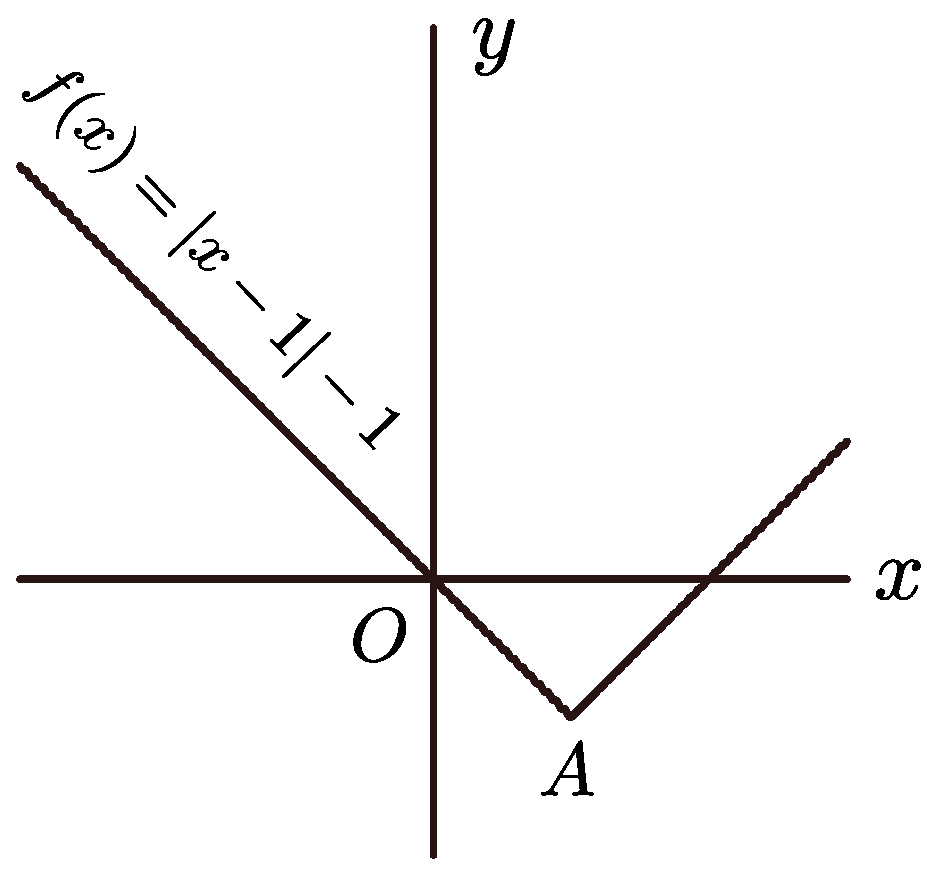
\includegraphics[scale=0.35]{figure.eps} 
\end{center} 

\newcard 

\begin{center}
  \begin{tabular}{NN}
   \toprule
   & \text{Value} \\
   \midrule 
   \lim_{x\to 1^-} f(x) & -1 \\ 
   \midrule 
   \lim_{x\to 1^+} f(x) & -1 \\
   \midrule 
   f(1) & -1 \\ 
    \bottomrule
  \end{tabular}
\end{center}

And hence, $f(x)$ is continuous at $x = 1$ 


\newcard 

The following table shows the values that we should be looking at to ascertain continuity at $x=1$ for $f(x)$ (as defined previously) 

\begin{center}
  \begin{tabular}{NNN}
   \toprule
   & \text{Expression} & \text{Value} \\
   \midrule 
   \lim_{x\to 1^-} f(x) & \lim_{x\to 1^-} (-x) & -1 \\ 
   \midrule 
   \lim_{x\to 1^+} f(x) & \lim_{x\to 1^+} (x-2) &  -1 \\
   \midrule 
   f(1) & (x-2) & -1 \\ 
    \bottomrule
  \end{tabular}
\end{center}

And as $\lim_{x\to 1} f(x) = f(1)$, therefore $f(x)$ is continous at $x=1$ 

\newcard 

\[ \qquad \lim_{x\to 1^-} f'(x) \neq \lim_{x\to 1^+} f'(x) \]
Hence $f(x)$ is \underline{not} differentiable at $x=1$ 

\newcard 

\[ \qquad \lim_{x\to 1^-} f'(x) = \lim_{x\to 1^+} f'(x) \]
Hence $f(x)$ is differentiable at $x=1$ 
 
\newcard 

Just by looking at the plot of $f(x)$ we made earlier, one can see that 
the \underline{rate of change} of $f(x)$ -- that is $f'(x)$ -- is not the same for $x\geq 1$ and $x < 1$ \newline 

But more formally 
\begin{center}
  \begin{tabular}{NN}
   \toprule
        & f'(x) \\
   \midrule 
   x \geq 1 & \ddx (x-2) = 1 \\
    \midrule 
    x < 1 & \ddx (-x) = -1 \\
    \bottomrule
  \end{tabular}
\end{center}

Hence, $f(x)$ is continuous \underline{but not} differentiable at $x =1$ 
\end{document}